\section{Design}

\subsection{Overordnet System Design}
\noindent Dette afsnit repræsenterer hvordan modulerne ønskes at kommunikere med hinanden, samt forsøger at give et overblik over, hvor meget der kommunikeres mellem modulerne i de forskellige stadier. Der vil i dette afsnit indgå 2 User stories til at repræsentere systemets design. Disse User Stories er relevante for design, da de involverer alle moduler samtidigt og giver et indblik i kommunikationen på tværs af systemet. For at se flere User Stories og hvordan de vil virke i systemet se bilag \parencite[][Section 8]{TekniskBilag}.

\noindent Herunder ses et sekvensdiagram for User Story 15 og 18, nemlig Save og Load game. Her ses hvordan det ønskes at de forskellige moduler kommunikerer på tværs af systemet, når en bruger at hente eller gemme data fra/i databasen.
\begin{figure}[H]
\centering
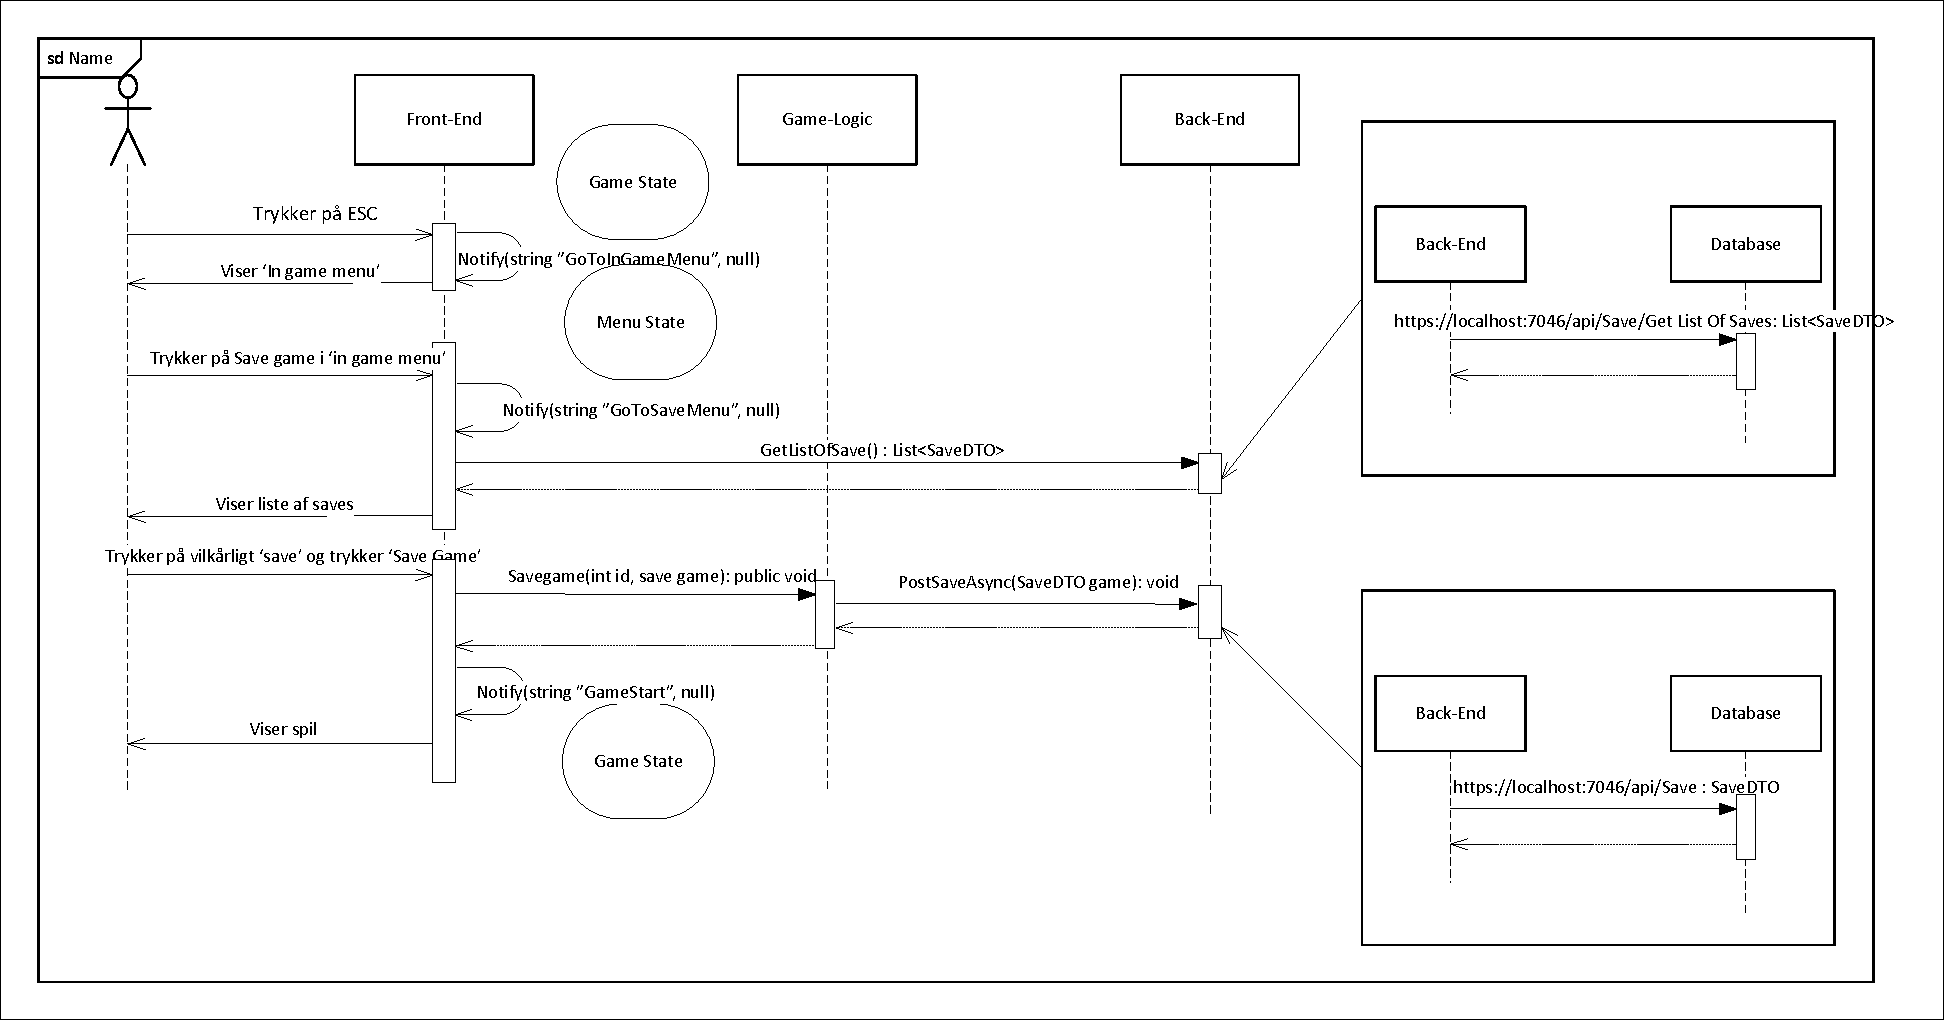
\includegraphics[width = \textwidth]{02-Body/Images/Arkitektur-SDSaveGame}
\caption{SD diagram for User Story 15 " Save Game". Diagrammet viser hvordan det ønskes at systemet overordnet skal kommunikere på tværs af hinanden når en bruger skal gemme sit aktuelle save}
\label{fig:Arkitektur-SD-SaveGame}
\end{figure}

\begin{figure}[H]
\centering
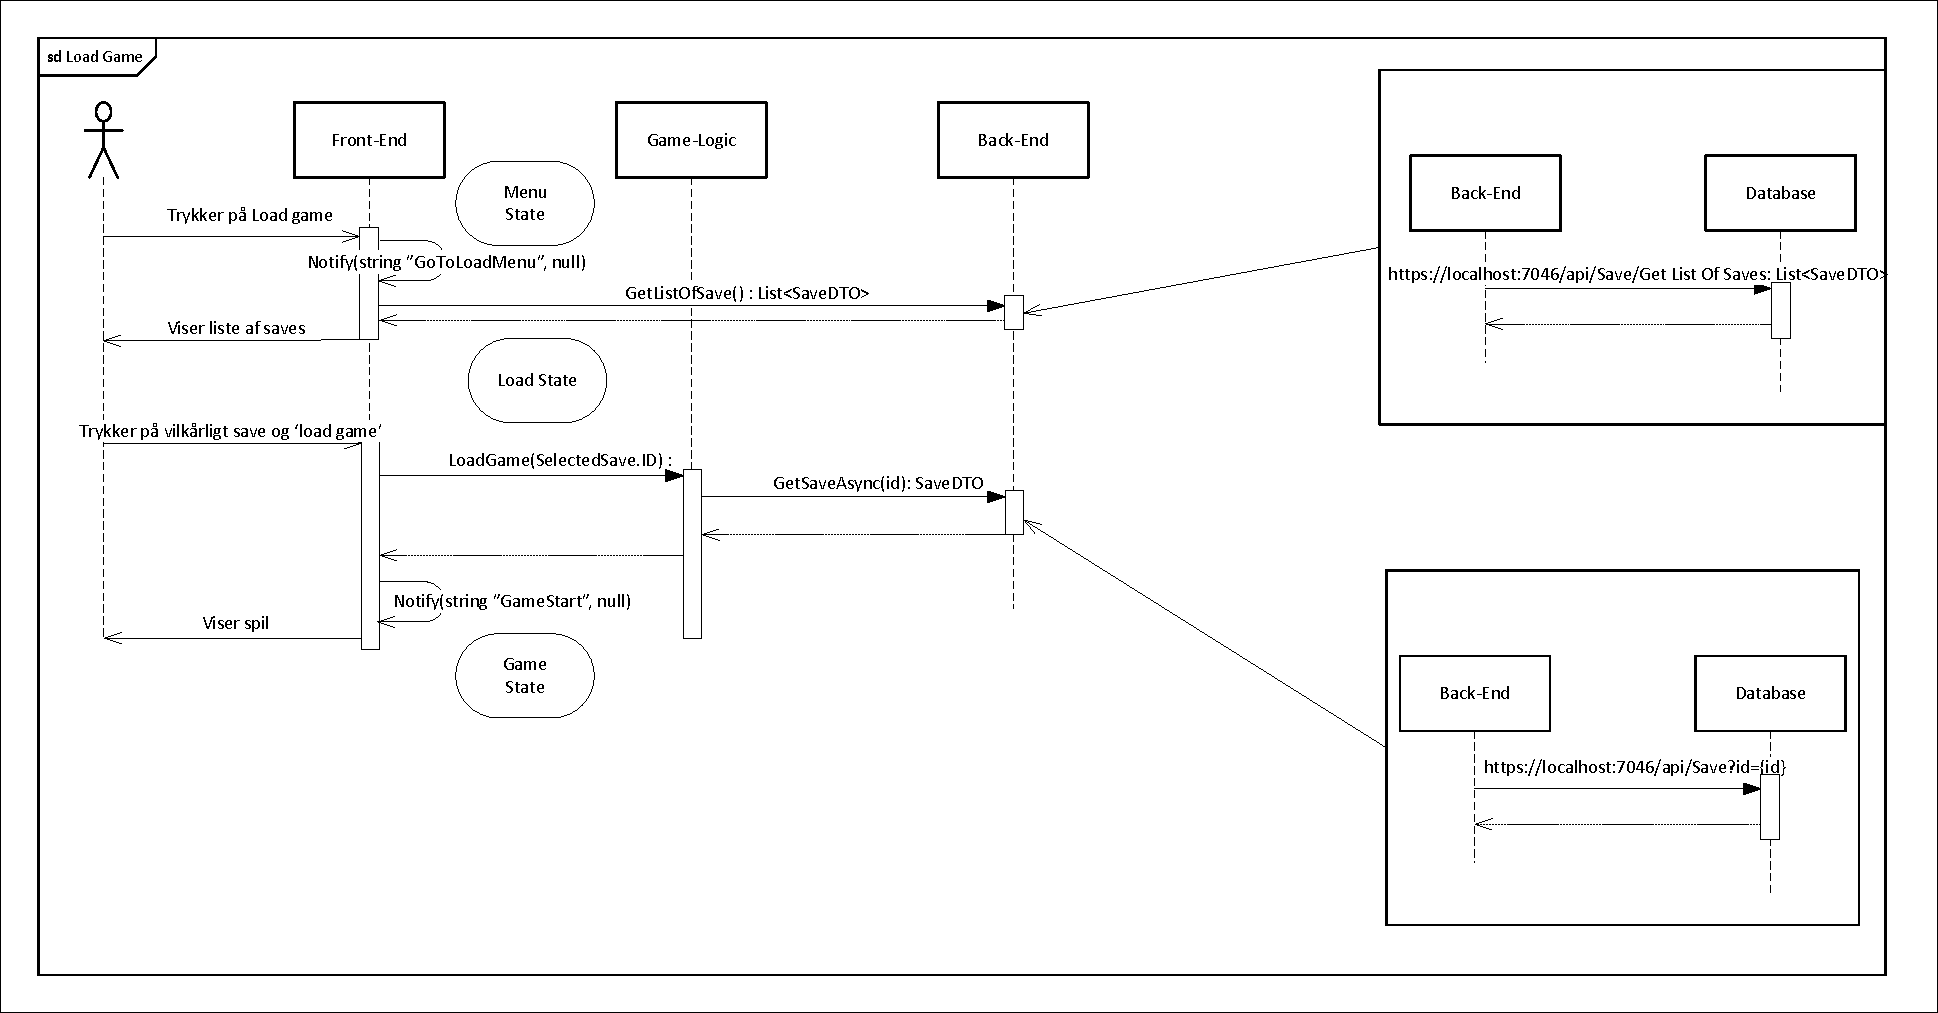
\includegraphics[width = \textwidth]{02-Body/Images/Arkitektur-SDLoadGame}
\caption{SD diagram for User Story 18 "Load Game". Diagrammet viser hvordan systemet overordnet skal kommunikere på tværs når bruger skal loade sit aktuelle save. }
\label{fig:Arkitektur-SD-LoadGame}
\end{figure}


\subsection{Front-end Design}
\label{ssec:FE Design}

Inden arbejdet på Front-end arkitekturen begyndte, er der blevet lavet en teknologiundersøgelse se Tekniskbilag (sektion 6.1), om hvilket udviklingsværktøj Front-enden og derigennem spillet skulle udvikles i. Baseret på denne teknologiundersøgelse er der blevet valgt, at spillet vil blive udviklet i et .NET framework. Dette valg er blandt andet truffet, da dette framework passer bedre med den opdeling af arbejde der er lavet i projektgruppen, altså opdelingen af Frontend og Backend. For andre grunde, se Tekniskbilag (sektion 6.1), hvor flere fordele og ulemper for både unity og .NET frameworket er sat op.\\

\noindent Spillets Front-end består af en række menuer, samt selve spil viewet. Spillet skifter så mellem disse forskellige menuer og views i samme vindue, således at brugeren får en flydende overgang.
Det primære spil-vindue er room view, et mock-up af dette view kan se på \autoref{fig:Design-FE-mockup-room}. Her præsenteres spilleren for en beskrivelse af det rum de er i, samt hvilke elementer i rummet de kan interagere med. Der vises også et kort over banen. Kortet viser kun de rum spilleren allerede har været i, mens resten holdes skjult. Når brugeren så besøger et nyt rum, kan dette ses selvom spilleren forlader rummet. Dette lader spilleren udforske og oplåse hele kortet.\\
En række knapper nederst i højre hjørne på skærmen giver spilleren mulighed for at interagere med spillet. Fire knapper ("Go {North/West/South/East}") lader spilleren gå fra et rum til et andet. Ikke alle rum har forbindelse til alle sider, så det er f.eks. ikke altid muligt at trykke på "Go North". Kortet og rum beskrivelsen fortæller hvilken vej det er muligt at bevæge sig i.\\
Udover de fire retningsknapper er der et antal andre knapper. Disse bruges til at gemme spillet, gå til menuer, samt interagere med elementerne i rummet. Det specifikke antal og deres funktion er afhængig af den præcise implementering.\\

\noindent For at læse mere om spillets andre menuer og views se Tekniskbilag (sektion 8.2)

\begin{figure}[H]
\centering
\includegraphics[width = \textwidth]{02-Body/Images/RoomMockup.PNG}
\caption{Et mockup af det primære spil vindue. Tekst øverst i venstre side af skærmen giver en beskrivelse af det rum spilleren er i, samt en liste af elementer i rummet som spilleren kan interagere med. Øverst til højre vises et billede af banen. Spilleren interagerer med spillet via knapper nederst i højre hjørne. Knapperne "Go {North/West/South/East}" fører spilleren ind i et andet rum, mens de resterende knapper (markeret "Button") bruges til andre funktionaliterer i spillet.}
\label{fig:Design-FE-mockup-room}
\end{figure}


\subsection{Game Engine design}
\label{sec:GameEngineDesign}

\noindent Spillets logik styres fra game engine, der består
af de komponenter, som modellere spillets verden og dens 
logik. Af disse komponenter er Game Controlleren, Combat Controlleren,
Room, og Player de mest essentielle.

\begin{figure}[H]
  \centering
  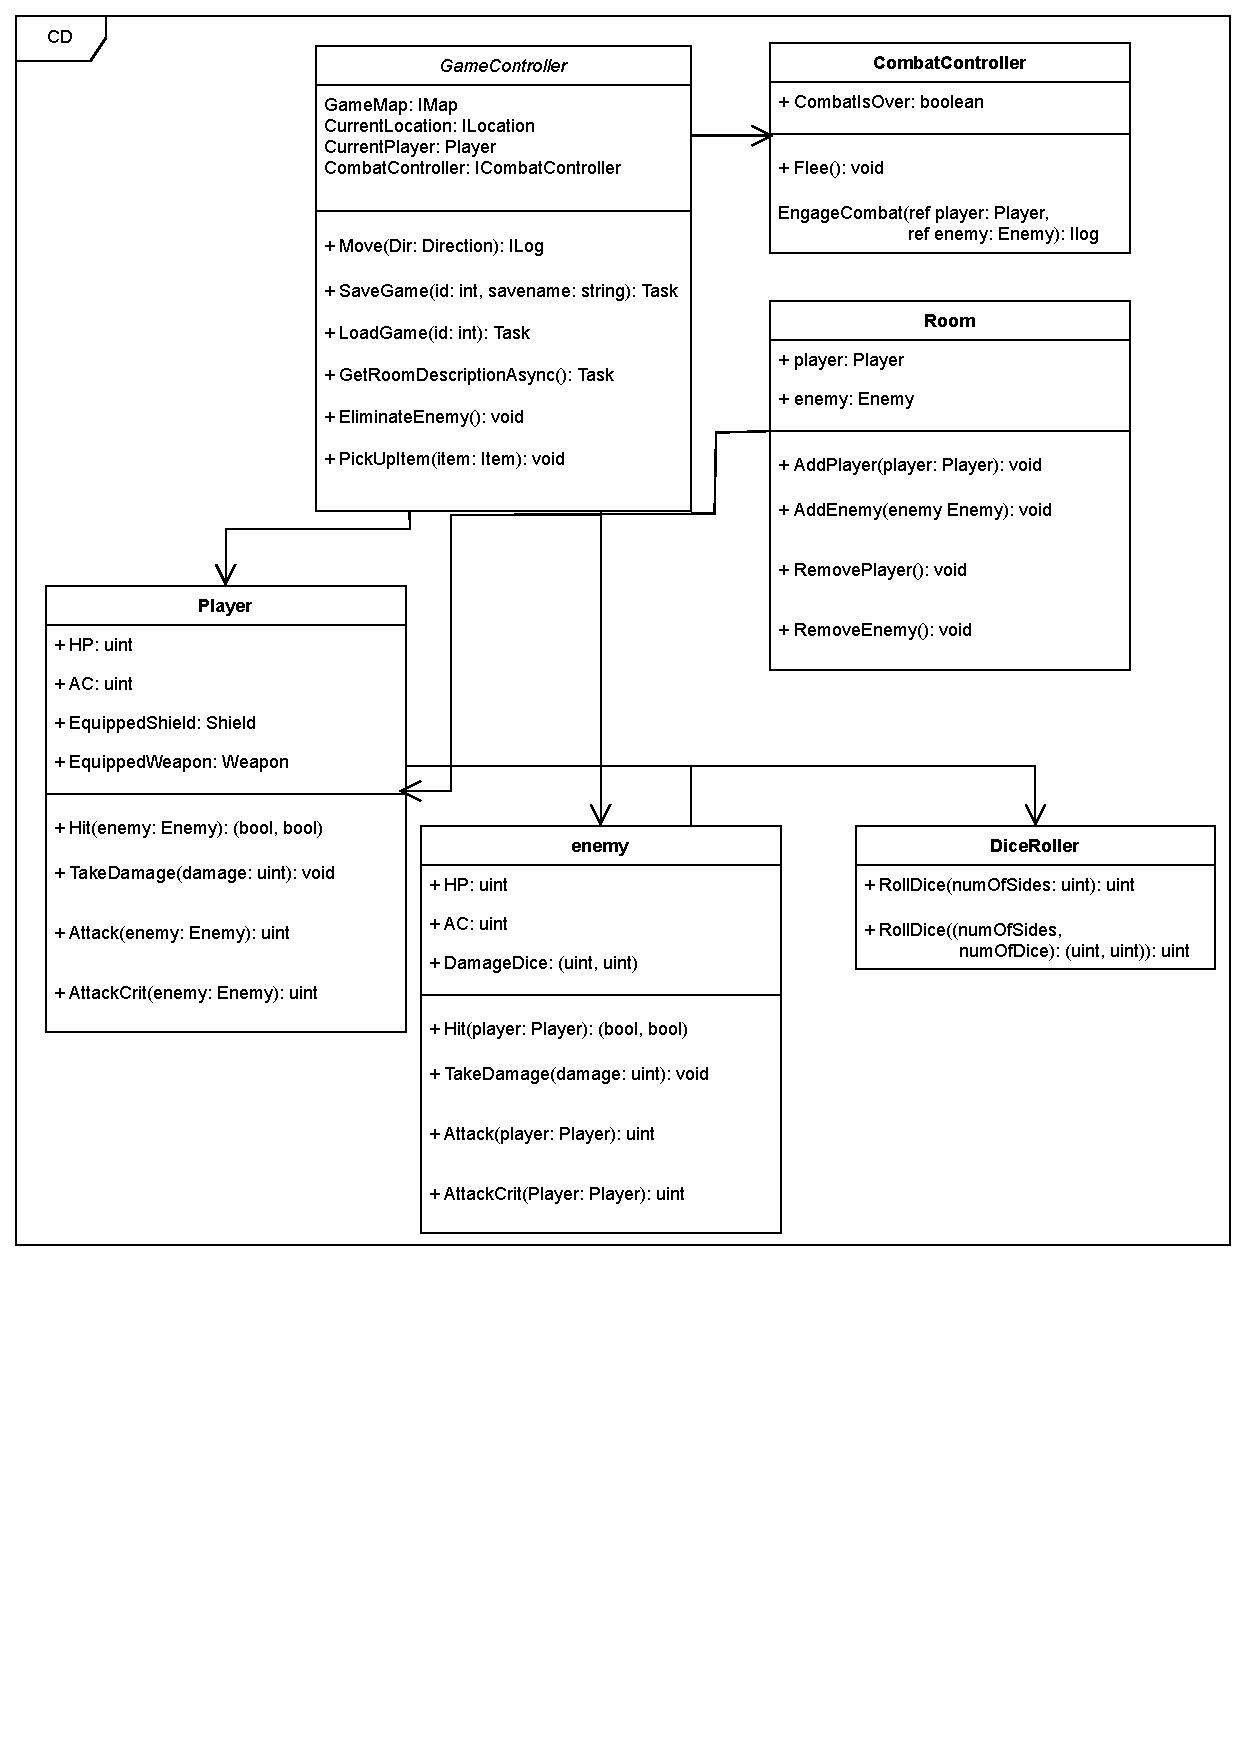
\includegraphics[width=\textwidth, trim = 0 9cm 0 0]{02-Body/Images/CoreClassDiagram.pdf}
  \caption{De vigtigste elementer af game engine og deres 
           relationer til hinanden. Der er her ikke vist 
           interfaces, men lagt fokus på de kritiske elementer
           som de er implementeret.}%
  \label{fig:CoreDiagram}
\end{figure}

\subsubsection{Game Controller}
Game Controlleren styre alle UI funktionaliteter, når brugeren
trykker på en knap, der påvirker spillets state, gøres dette
gennem game controlleren. Game controlleren instantieres når
et spil startes; hvilket danner et map \parencite[Section 8.3.1][]
{TekniskBilag}, spilleren kan navigere rundt på. 

Game controlleren tillader at spilleren kan bevæge sig mellem
spillets forskellige rum \parencite[Section 7.3.1][]{TekniskBilag} 
i overenstemmelse med spillets map layout. Skulle spilleren forsøge at
bevæge sig i en retning, der ikke er tilladt ifølge map layoutet bliver 
spilleren stående i det nuværende rum.

Skulle spilleren bevæge sig ind i et rum med et ``item'', styre 
game controlleren spillerens evne til at inteagere med ``itemet''.
Spilleren har evenen til at samle ``items'' op, og derved øge deres
stats.

I det tilfælde, at spilleren bevæger sig ind i et rum med en modstander,
giver game controlleren spilleren evnen til at bekæmpe fjenden eller
flygte fra denne. Game controlleren gør dette ved at kalde combat controlleren,
som håndtere kamp i spillet.

\subsubsection{Combat Controller}
Combat controlleren håndterer spillets logik, i det omfang det relatere sig til
kamp mellem spilleren og en fjende \parencite[Section 7.3.3][Figur 17]{TekniskBilag}.

\noindent Combat i spillet afvikles ved hjælp af flere simulerede terningekast (RNG) se dicerollern,
i \autoref{fig:CoreDiagram} der afgører både om spilleren/fjenden rammer fjenden/spilleren 
og hvor meget skade fjende/spilleren modtager. Spillets ``items'' har indflydelse
på vægtningen af disse simulerede terningekast, og kan hjælpe spilleren med at ramme og skade 
modstanderen. ``items'' kan også gøre det svære for fjenden at ramme spilleren.

Spilleren kan efter hvert sæt af terningekast vælge at forsætte kampen eller
flygte. Skulle spillerens liv nå nul, dør spilleren og spillet er færdigt.

\subsubsection{Room}
Et ``Room'' eller rum er en diskret delmængde af spillets verden, som kan indeholde
spilleren, fjender og forskellige genstande. ``Room'' er kun ansvarlig for at tilføje
og fjerne spilleren og fjender for rummet se \autoref{fig:CoreDiagram}. Ikke desto mindre
kunne spilleren ikke navigere verden uden existensen af disse diskrete områder.

\subsubsection{Player}
Spillerens karakter (PC) repræsenterer spilleren i spillet. Dette komponent er ansvarlig for at
holde styr på spillerens tilstand i spillet og giver spilleren evnen til at forsvare
sig selv i kamp. Denne simulerer en spillers forsøg på at ramme en fjende, skade en 
fjende og opdatere spilleren liv, forsvar og ``items'' undervejs i spillet 
\parencite[Section 8.3.2][]{TekniskBilag}.


\newpage

\subsection{Backend Design}
\label{ssec: Backend Design}

I det følgende afsnit beskrives design overvejelser i forbindelse med udviklingen af systemets backend Web Api. Afsnittet vil give et overblik over hvilke resources/routes Web api’et stiller til rådighed. Efterfølgende forklares hvordan Data transfer objects vil blive anvendt, hvordan Authentication og Autherization vil blive håndteret, samt hvordan passwords vil blive hashed. Hertil vil en BackEndController klasse, som skal bruges på client siden blive redegjort for. Tilslut præsenteres applikationsmodeller over controller klasserne for de relevante User Stories, som består af en række sekvens og klasse diagrammer.\\

\subsubsection{Analyse konklusion}
I dette projekt vil give bedst mening at anvende mulighed 1 baggrunden for denne beslutning kan ses i \autoref{ssec: Teknisk Analyse Backend} med en backend bestående af ASP.NET og EF Core. Her fåes nemlig muligheden for at separere data resourcerne fra resten af applikationen samtidig med vi for en mere sikker og pålidelig håndtering af brugere samtidig med EF Core stadig understøttes til kommunikation med databasen i gennem LINQ. \cite{Language Integrated Query}\\


\subsubsection{Routes}
Applikationens nødvendige routes kan inddeles i to under grupper ”Save”, som indeholder routes relateret til game state og ”User”, som indeholder routes relateret til brugeren. Alle routes som omhandler game state skal authorizes, mens routes, som omhandler brugeren tilader anonyme forespørgelser. Nedenfor er givet en oversigt over de forskellige routes med en tilhørende beskrivelse.\\

\textbf{Save:}\\
\begin{itemize}
\item GET: /api/Save
Denne route henter et sepcifikt gemt game state fra databasen, for den bruger som er logget ind.
\item POST: /api/Save\\
Denne route sender et scecifikt game state til databasen, for den bruger som er logget ind.
\item GET: /api/Save/Get List Of Saves\\
Denne route henter en liste af game states, for den bruger som er logget ind. 
\item GET: /api/Save/Get Room Description\\
Denne route henter en beskrivelse af det valgt rum i spillet.
\end{itemize}

\textbf{User:}\\
\begin{itemize}
\item POST: /api/User/Register\\
Denne route registrerer en ny bruger ved at gemme oplysninger om denne i databasen, og returnerer en JWT token. Når en bruger bliver registreret får den tildelt 5 pladser i databasen til game states.
\item POST: /api/User/Login\\
Denne route logger en bruger ind ved at tjekke bruger oplysninger med dem, som er registreret i databasen, denne route returnerer også en JWT token.
\end{itemize}

\subsubsection{Data Transfer Object:}

De data objekter som gemmes i SQL databasen vil indeholde nogle navigational properties, som bruges til at query data’en og til at opretter relationer mellem objekterne. Da disse properties ikke har nogen relevans for clienten oprettes der følgende DTO’er for modellerne User og Save som ses på \autoref{fig:Design-Backend-DTO}\\

\begin{figure}[H]
\centering
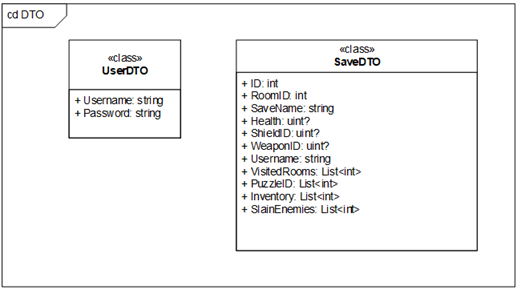
\includegraphics[width = \textwidth]{02-Body/Images/Backend_DTO.PNG}
\caption{klasse diagram over DTO'er for User og Save}
\label{fig:Design-Backend-DTO}
\end{figure}

På den måde kan man sikre at kun den nødvendige data sendes til clienten.\\

\subsubsection{Authentication/Authorization med JWT Token}
JWT (Jason Web Token) er et JSON object, som bruges til at validere (Authenticate), og til at afgøre hvorvidt en client har adgang til den givne data (Authorizing). En token består af tre dele en header, en payload og en signature.\\

\textbf{Header:}\\
Headeren består af en type og en hashing algoritme, typen vil for dette system være ”JWT” og algortimen vil være ”HmacSha256”.\\

\textbf{Payload:}\\

Payloaden indeholder såkaldte claims, der findes tre typer af claims reserved, public og private. Reserved er en række prædefineret claims som kan bruges til eksempelvis at sætte en tidsbegrænsning på den gældende. Public og private claims kan indeholde noget information omkring brugeren. I dette system benyttes private claims til at indeholde brugerens username, som så kan bruges til at genkende hvem den aktuelle token tilhører ved en forespørgsel.\\

\textbf{Signature:}\\
Signature bruges til at verificere hvem som er afsender af JWT’en, og til sikre at den ikke er blevet ændret undervejs. Her samles header, payload og en ”secret” som er en hemmelig string af tegn, kun Web Api'et kender.
For at generere denne token implementeres en funktion, som opretter en token efter de forhold som er beskrevet ovenfor.\\


\subsubsection{Hashing}
\label{sssec: Hashing}
Under design fasen blev det besluttet at anvende hashing til at gemme en brugers password i databasen, for at øge sikkerheden. Sikkerhed var ellers ikke prioteret i vores MoSCoW analyse \autoref{ssec:MOSCOW}, for denne udgave af spillet.
Hashing af passwords går ud på at kryptere det gemte password i databasen. Det skal krypteres således at det ikke er muligt at dekryptere, samtidig med at det stadig kan valideres om det er et korrekt password, der modtages af en client. Når et password hashes anvendes et såkaldt ”salt”, som er en tilfældigt genereret string kobineret med password’et.\\

Til at Hashe passwords med anvendes Bcrypt \cite{Bcrypt}, dette library stiller hashing af passwords til rådighed. Der findes en C\# udgave kaldet Bcrypt.Net  som vil blive anvendt. Helt præcist er det funktionen HashPassword(”password”, BcryptWorkfactor), denne funktion skal have en BcryptWorkfactor, hvilket er et tal der siger noget om hvor mange iterationer Bcrypt vil bruge på at generere det ”salt” til at hashe password’et med. Her anbefales det at bruge en værdi på 11, da det generelt set anses som tilstrækeligt niveau hvad angår sikkerhed.
Funktionen verify(”password”, hashedpassword) bruges til at verificere om et givent password svare til dets krypterede udgave.\\

\subsubsection{BackEndController på client siden}
Til brug af clienten for at tilgå backenden, skal der bruges en BackendController klasse, dennes ansvar vil være at udføre HTTP request/responses, og vil indeholde en funktion for hvert endpoint.\\
 
Klassen vil gøre brug af en HttpClient som er en klasse .Net stiller til rådighed til at håndtere HTTP request/responses. Da backenden kræver en JWT for at få adgang til endpoints, hvad angår loading og saving af game state, skal clienten også gemme JWT for den bruger som er logget ind, således at den kan blive sendt med de forskellige requests.


\subsection{Applikationsmodeller}
I dette afsnit gennemgåes applikationsmodeller for de enkelte user stories, der udarbejdes sekvensdiagrammer for at beskrive funktionalitet og klasse diagrammer til at beskrive indeholdet og sammen spillet imellem klasserne. Applikationsmodellerne deles op efter controllere, en for UserControlleren og en for SaveControlleren. Fokuset vil her ligge på controller klasserne, for en beskrivelse af DAL komponenterne henvises til database design afsnitet \autoref{ssec:DB Design}.\\

\subsubsection{Applikationsmodel User Controller}
\textbf{User Story 1: Log in}\\
Når clienten udfører en HTTP request med URL’en : ” https://localhost:7046/api/User/Login”, udføres følgende aktioner som fremgår af sekvensdiagrammet på \autoref{fig:Design-Backend-Sekvens-1}\\ 

\begin{figure}[H]
\centering
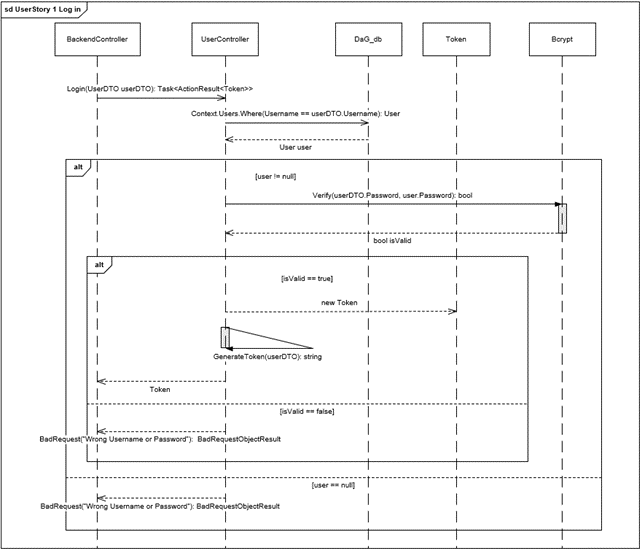
\includegraphics[width = \textwidth]{02-Body/Images/Backend_sekvens_1.PNG}
\caption{Sekvensdiagram som viser funktionaliteten i User Story 1 Log in}
\label{fig:Design-Backend-Sekvens-1}
\end{figure}

Authentication controlleren fra C3 modellen hedder her “UserController” og har til opgave at gøre det muligt for en bruger at registrere sig og logge ind. Login implementeres i Login() funktionen, som er det endpoint clienten kalder for at logge ind. Her bliver der tjekket om det indtastede brugernavn findes i databasen. Hvis brugernavnet findes, så bliver adgangskoden tjekket med funktionen verify fra Bcrypt klassen, og passer den, bliver der returneret en JWT token. Hvis brugernavnet derimod allerede eksiterer eller adgangskoden ikke er korrekt retuneres en fejlmeddelse.\\

\textbf{User Story 2: Opret Bruger}\\
Når clienten udfører en HTTP request med URL’en : ” https://localhost:7046/api/User/Register”, udføres følgende aktioner som fremgår af sekvensdiagrammet på \autoref{fig:Design-Backend-Sekvens-2}\\

\begin{figure}[H]
\centering
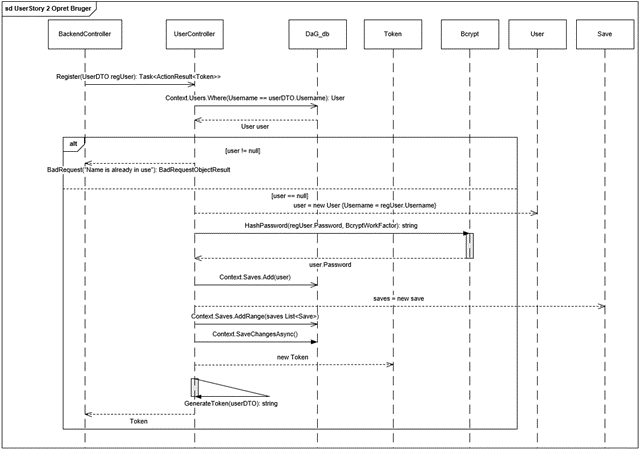
\includegraphics[width = \textwidth]{02-Body/Images/Backend_sekvens_2.PNG}
\caption{Sekvensdiagram som viser funktionaliteten i User Story 2 Opret Bruger}
\label{fig:Design-Backend-Sekvens-2}
\end{figure}

For at kunne logge ind skal det være muligt at oprette en bruger til dette laves en Register(UserDTO regUser) funktion. Denne starter med at checke om brugernavnet er optaget. Er den det, returneres der en fejlmeddelelse, og ellers registreres brugeren. Dernæst bliver det valgte kodeord ”hashed”, således at der opnås en vis sikkerhed i systemet. Når der oprettes en ny bruger skal denne have tildelt 5 pladser i databasen til sine gemte spil, dette sker ved at der oprettes en liste af saves der indeholder 5 nye saves, disse gemmes med contexten i SQL databasen. Hvis alt går godt retuneres en JWT token.\\

\textbf{Samlet Klasse diagram over User Story 1 og 2}\\

På \autoref{fig:Design-Backend-Klasse-1-2} kan ses en oversigt over de klasser, metoder og attributter, som anvendes i udførelsen af User story 1 og 2. Hertil anvendes også klassen Bcrypt som ikke er taget med, da den blot er brugt udefra, detaljer om Bcrypt kan ses i afsnitet ovenover \autoref{sssec: Hashing}.\\

\begin{figure}[H]
\centering
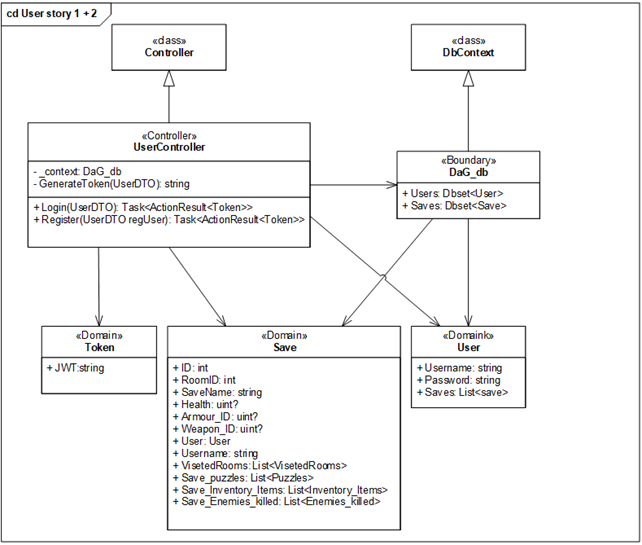
\includegraphics[width = \textwidth]{02-Body/Images/Backend_klasse_1_2.PNG}
\caption{Samlet klasse diagram over User story 1 og 2}
\label{fig:Design-Backend-Klasse-1-2}
\end{figure}

\subsubsection{Applikationsmodel Save Controller}
\textbf{User Story 7: Exit Menu -\g Save and Exit}\\
Load/save controlleren fra C3 modellen er blevet til en enkelt controller, som kaldes for ”SaveController”. Denne controller har til ansvar at gemme et spil, men samtidig også være i stand til at kunne hente gemte spil, altså at loade dem.
Når clienten udfører en HTTP request med URL’en : ” https://localhost:7046/api/Save”, udføres følgende aktioner som fremgår af sekvensdiagrammet på \autoref{fig:Design-Backend-Sekvens-7}\\

\begin{figure}[H]
\centering
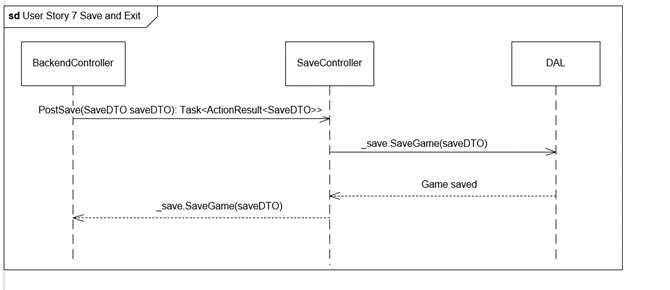
\includegraphics[width = \textwidth]{02-Body/Images/Backend_sekvens_7.PNG}
\caption{sekvensdiagram over User Story 7 Save and Exit}
\label{fig:Design-Backend-Sekvens-7}
\end{figure}

Der bruges en httpPost funktion kaldet PostSave som gemmer et nyt spil i databasen ved at ligge det modtagene gamestate fra parameter listen ind i et funktionskald SaveGame() i DAL klassen, som så sørger for at gemme spillet i databasen på den korrekte måde.\\

\textbf{User Story 17: Exit Menu -\g Save and Exit}\\

Når clienten udfører en HTTP request med URL’en : ” https://localhost:7046/api/Save/Get List Of Saves”, udføres følgende aktioner som fremgår af sekvensdiagrammet på \autoref{fig:Design-Backend-Sekvens-17}\\

\begin{figure}[H]
\centering
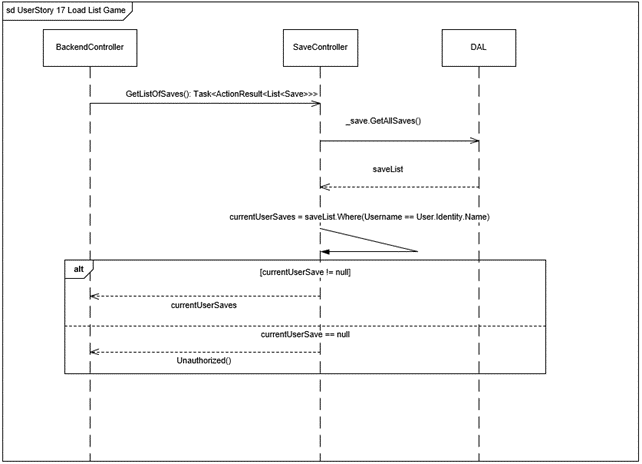
\includegraphics[width = \textwidth]{02-Body/Images/Backend_sekvens_17.PNG}
\caption{Sekvensdiagram over User Story 17 Main Menu -\g Load List Game}
\label{fig:Design-Backend-Sekvens-17}
\end{figure}

Da vi gerne vil gøre det muligt at have 5 save games pr. profil, skal det naturligvis være muligt at kunne vælge mellem de forskellige saves, til dette laves funktion GetListOfSaves(). Clienten kalder her GetListOfSaves() som er et HttpGet endpoint, denne funktion henter alle saves i DAL klassen ved at kalde GetAllSaves(). SaveController finder så de gemte spil i listen hvor brugernavnet passer med den burger, som er logget ind ved brug af User.Identity som stilles til rådighed af ControllerBase klassen, her i kan claims for den nuværende JWT nemlig findes.\\

\textbf{UserStory 18 : Main Menu -\g Load Game -\g Load}\\
Når clienten udfører en HTTP request med URL’en :” https://localhost:7046/api/Save?id={id}”, udføres følgende aktioner som fremgår af sekvensdiagrammet på \autoref{fig:Design-Backend-Sekvens-18}\\

\begin{figure}[H]
\centering
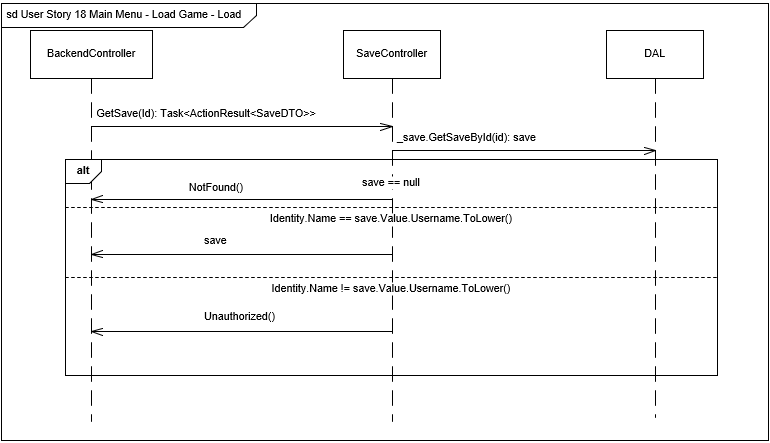
\includegraphics[width = \textwidth]{02-Body/Images/Backend_sekvens_18.PNG}
\caption{Sekvens diagram over User story 18 Main Menu -> Load Game -> Load}
\label{fig:Design-Backend-Sekvens-18}
\end{figure}

\textbf{User Story 19 : Main Menu -\g Load Game -\g Delete Game}\\

Under design fasen blev det besluttet at overskrive gemte saves fremfor at slette og lave et nyt, da et saves Id på den måde ikke ændret sig i databasen når man lavede et nyt save. Derfor er User story 19 som omhandler Delete game ikke taget med i design fasen.\\

\textbf{Samlet klasse diagram over User story 7, 17 og 18}\\
Et Samlet klasse diagram for User story 7, 17 og 18 kan ses på \autoref{fig:Design-Backend-Sekvens-7-17-18}\\

\begin{figure}[H]
\centering
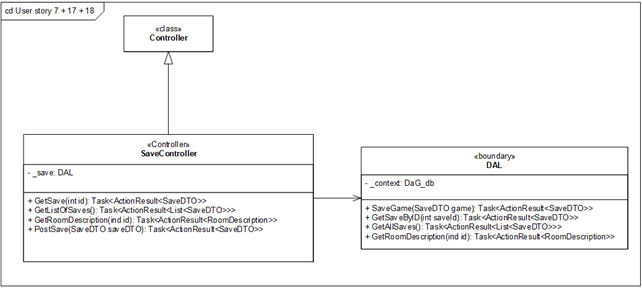
\includegraphics[width = \textwidth]{02-Body/Images/Backend_klasse_7_17_18.PNG}
\caption{Samlet klasse diagram for User story 7, 17 og 18}
\label{fig:Design-Backend-Sekvens-7-17-18}
\end{figure}

Udover de funktioner som bliver brugt i User stories, tilføjes der er en funktion GetRoomDescription, som blot henter en beskrivelse af det rum brugeren befinder sig i.\\


\subsubsection{Konklusion}

Backenden er blevet designet såldedes at den kan håndtere alle de nødvendige kald for at opfylde user stories omkring brugere og gemte spil, dette er beskrevet igennem appilationsmodeller. JWT tokens anvendes til Authentication og Authorization. Til hashing af passwords anvendes Bcrypt. Hertil er BackendControlleren klassen blevet introduceret på clienten, som står for HTTP request/response.\\ 


\newpage

\subsection{Software Design DAL Design}
På \autoref{fig:DAL-Klasse-7-17-18} herunder ses klassediagrammet over backend DAL, som benyttes til database access. 
Som det kan ses på diagrammet, indeholder DAL en database context, som benyttes til at forbinde backend applicationen til databasen. 
Derudover består DAL af fire overordnede funktioner, hvoraf de 3 tilhører en user story. 
Den sidste funktion benyttes når vi starter spillet, til at lave rumbeskrivelser.\\

\begin{figure}[H]
\centering
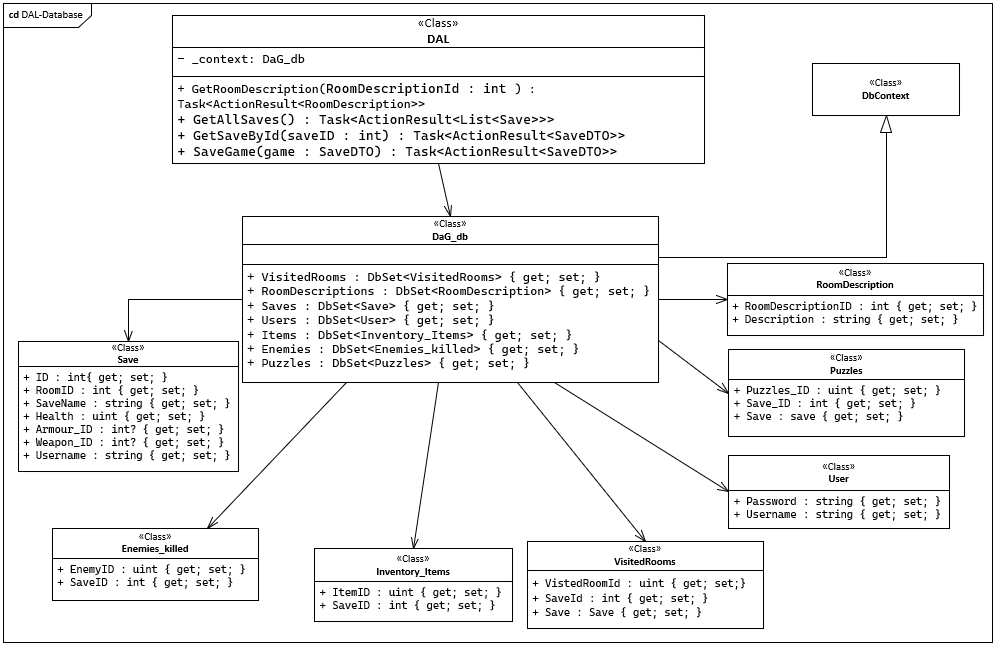
\includegraphics[width = \textwidth]{02-Body/Images/DAL-Database/DAL-DB-CD.PNG}
\caption{Samlet klasse diagram for User story 8, 15, 17 og 18 med DAL db context og entitetsklasser.
For læseligheden er DAL klassen ikke forbundet til forskellige entitetsklasser selvom disse benyttes.}
\label{fig:DAL-Klasse-7-17-18}
\end{figure}

Følgende funktion som beskrives på \autoref{fig:DAL-Sekvens-RumBeskrivelser} benyttes når spil klienten startes, da beskrivelser af rum ikke ændre sig gennem spillets levetid, i den nuværende itteration.\\

\begin{figure}[H]
\centering
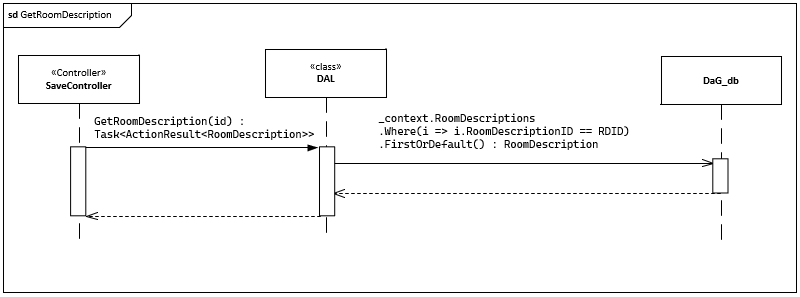
\includegraphics[width = \textwidth]{02-Body/Images/DAL-Database/RoomDescriptionSd.PNG}
\caption{Sekvensdiagram om læsning af en rumbeskrivelse}
\label{fig:DAL-Sekvens-RumBeskrivelser}
\end{figure}

Navn: GetRoomDescription \\
Parametre: int RoomDescriptionId \\
Returtype: Task\l ActionResult\l RoomDescription\g\g\\
Beskrivelse: Denne funktion finder og returnerer en beskrivelse for det valgte RoomDescriptionID. 
Dette kan også ses på sekvensdiagrammet på figur \autoref{fig:DAL-Sekvens-RumBeskrivelser}.


\subsubsection{User story funktioner}
De følgende 3 funktioner benyttes til udførelse af forskellige user stories.
Det drejer sig om:
\begin{itemize}
\item User story 15 – Save game
\item User story 8 - Save - No Combat  + User story 17 – Load game list 
\item User story 18 – Load game \\
\end{itemize}

Funktionen GetById benyttes til at udfører user story 18.
Her skal der loades et gemt spil, som brugeren nu ønsker at spille. 
Dette kan også ses på sekvensdiagrammet på \autoref{fig:DAL-Sekvens-18}.\\

\begin{figure}[H]
\centering
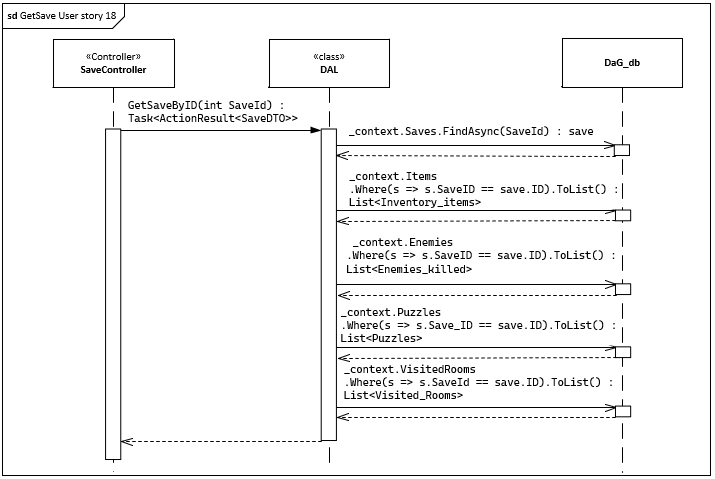
\includegraphics[width = \textwidth]{02-Body/Images/DAL-Database/GetSavesByIdSd.PNG}
\caption{Sekvensdiagram for user story 18 GetSaveById som beskriver queries til databasen for at hente et specifikt save og dens tilhørende information}
\label{fig:DAL-Sekvens-18}
\end{figure}

Funktionsbeskrivelse:\\
Navn: GetSaveById \\
Parametre: int saveID\\
Returtype: Task\l ActionResult\l SaveDTO\g\g\\
Beskrivelse: Denne funktion finder det save med det medsendte ID, samt tilhørende lister, indsætter værdier i et SaveDTO objekt, hvorefter det returneres.\\

Funktionsbeskrivelser og sekvensdiagrammer for de 2 andre user story funktioner kan findes i det tekniske bilag sektion 10.6
\subsection{Database Design}

Projektets database har gruppen valgt at hoste i lokal storage. Dette er valgt da der under semesterets forløbet opstod problemer med skolens licens af Microsoft produkter. For at undgå at komme ud for udfordringer med hosting senere i forløbet, blev der valgt at gå med den sikre løsning, at hoste databasen lokalt på enheden. Til dette benyttede gruppen et docker image, specifikt det samme image som blev benyttet i DAB undervisning, til vores SQL server.
%(https://docs.microsoft.com/en-us/sql/linux/quickstart-install-connect-docker?view=sql-server-ver15&preserve-view=true&pivots=cs1-powershell)
Hvis ikke der var problemer microsoft, havde gruppen i stedet valgt at lagre data på en cloud-based storage fremfor lokal storage.\\



For at kunne udarbejde et ER diagram til modellering af vores sql database skal vi start med at finde ud af hvilke krav vi har til og hvilke attributter vi ønsker at gemme i vores database.
Først og fremmest ønskede grupper at vi kunne gemme beskrivelserne af de forskellige rum, i spillets layout, for at formindske antallet af filer i klienten, og samtidigt gøre eventuelle senere tilføjelser nemmere.\\ 
Her benyttes rummets id som key, da vi ikke ønsker at man skal kunne oprette flere beskrivelser til samme rum. Diagrammet kan ses på \autoref{fig:ER-Roomdescription}.

\begin{figure}[H]
\centering
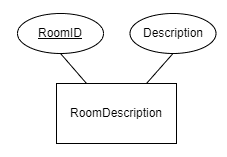
\includegraphics[width = 0.4\textwidth]{02-Body/Images/ER-RoomDescription.PNG}
\caption{ER diagram for Roomdescription. En beskrivelse består blot af en beskrivende string samt det tilhørende unikke rumid.}
\label{fig:ER-Roomdescription}
\end{figure}

Her efter kommer kravene til at kunne gemme et spil for en bruger. Her ønskede vi at man kunne stå et vilkårligt sted i spillet, med untagelse af en combat, og gemme spillet. Det skulle derefter være muligt for spilleren at loade spillet igen, hvorefter spillet er i samme stadie som man gemte det i.
ER diagrammet for at gemme et spil til en bruger på \autoref{fig:ER-GameSave}.
\begin{figure}[H]
\centering
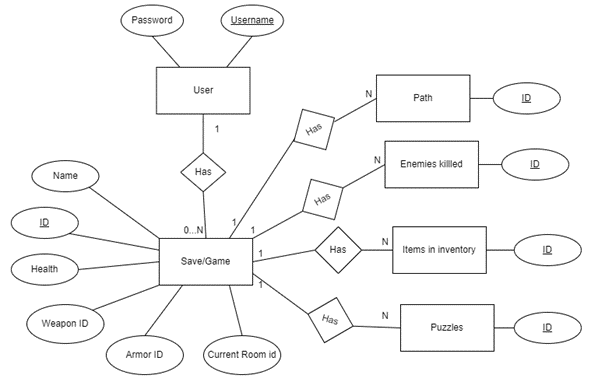
\includegraphics[width = \textwidth]{02-Body/Images/ER-GameSave.PNG}
\caption{ER Diagram til at gemme et spil til en specifik bruger. Her ses de forskellige informationer som skal til for at kunne gemme et helt spil}
\label{fig:ER-GameSave}
\end{figure}

Først og fremmest ønskede gruppen et bruger system, så eventuelle gemte spil kun tilhørte en bruger.
Der gemmes derfor en bruger entitet med et unikt brugernavn og et tilhørende password.
Sikkerhed på password og versalfølsomhed på brugernavnet håndteres af spillets backend.\\
En spiller skal derefter kunne gemme unikke 5 spil med forskellige oplysninger.
Restriktionen med max 5 forskellige spil pr. Bruger, håndteres ved at oprette 5 "tomme" gemte spil ved oprettelsen af en bruger.
Et af disse gemte spil overskriver derfor når vi gemmer. Der kan på denne måde ikke oprettes mere en 5 gemte spil pr. bruger.\\
I et gemt spil ønkede vi at gemme en række forskellige attributter for spilleren.
Første og fremmest får hver spil et unikt id som vi benytter til identifikation og at lave forhold mellem de forskellige tabeller.
Et gemt spil får et navn, valgt af brugeren, som gør det nemmere for brugeren at differentiere mellem de forskellige spil. \\ Dette navn skal være forskelligt fra de 4 andre gemte spil som tilhører samme bruger.\\
En spiller Health gemmes også, da man kan have taget skade efter en kamp.\\
Det gemmes også hvilket rum, spilleren står i når spillet gemmes, så vi loader korrekt tilbage. 
En spiller kan derudover også holde genstande, som armor og våben, i hånden eller i sit inventory. Dette gemmes også henholdsvist som en del af et spil og i en inventory liste tilhørende spillet. 

Tabellen med inventory har 2 atributter, et ID, som svarer til en bestemt genstand, og en reference til set SaveID. Denne parring er unik, da man ikke kan holde 2 af den samme genstand.\\
Tabellerne med Enemies og puzzles fungerer på samme måde. Her har hver enemy og puzzle i spillet et unikt id. Id’et gemmes i kombination med et saveId, som et unikt par, da man ikke kan vinde over samme enimy og løse samme puzzle flere gange.\\
Til slut ønskede vi at kunne vise spilleren de rum som allerede er blevet besøgt. Derfor gemmes der i path tabellen, for hvert spil, en unik kombination af saveID og besøgte rum id. Denne parring er unik da man blot behøver at besøge et rum en gang, før det er synligt på kortet. 

Der er i projektet oprettet klasser tilsvarende ER diagrammerne.
Forholdene mellem disse, samt keys, er opsat i DaG-db klassen og er skrevetved hjælp af fluentAPI. Dette kan ses i Implementationsafsnittet \autoref{Section: DB-Implementering}.

